
We've developed our methods by extending the basic intuition of \ocp. Since dynamic tensor decomposition pursues shorter time factor updates, this results low accuracy factorization when real-time data incomes. To optimize the speed accuracy problem, we'd like to trigger static decomposition method, \cpals while dynamic method like \ocp is being done.

\subsection{\em OnlineCP-trigger}
\textbf{Detection Approach}: \cpals activates whole temporal factor updates and enables high accuracy decomposition. Drastic data can be detected by calculating image error norm and its ratio between neighboring time steps. The moment for triggering \cpals is when temporal ratio of error norm for incoming data exceeds threshold.

\begin{align*}
    threshold < \frac{\norm{\tilde{\chi}_{i+1}-\chi_{i+1}}}{\norm{\tilde{\chi}_{i}-\chi_{i}}}
\end{align*}

\begin{center}
	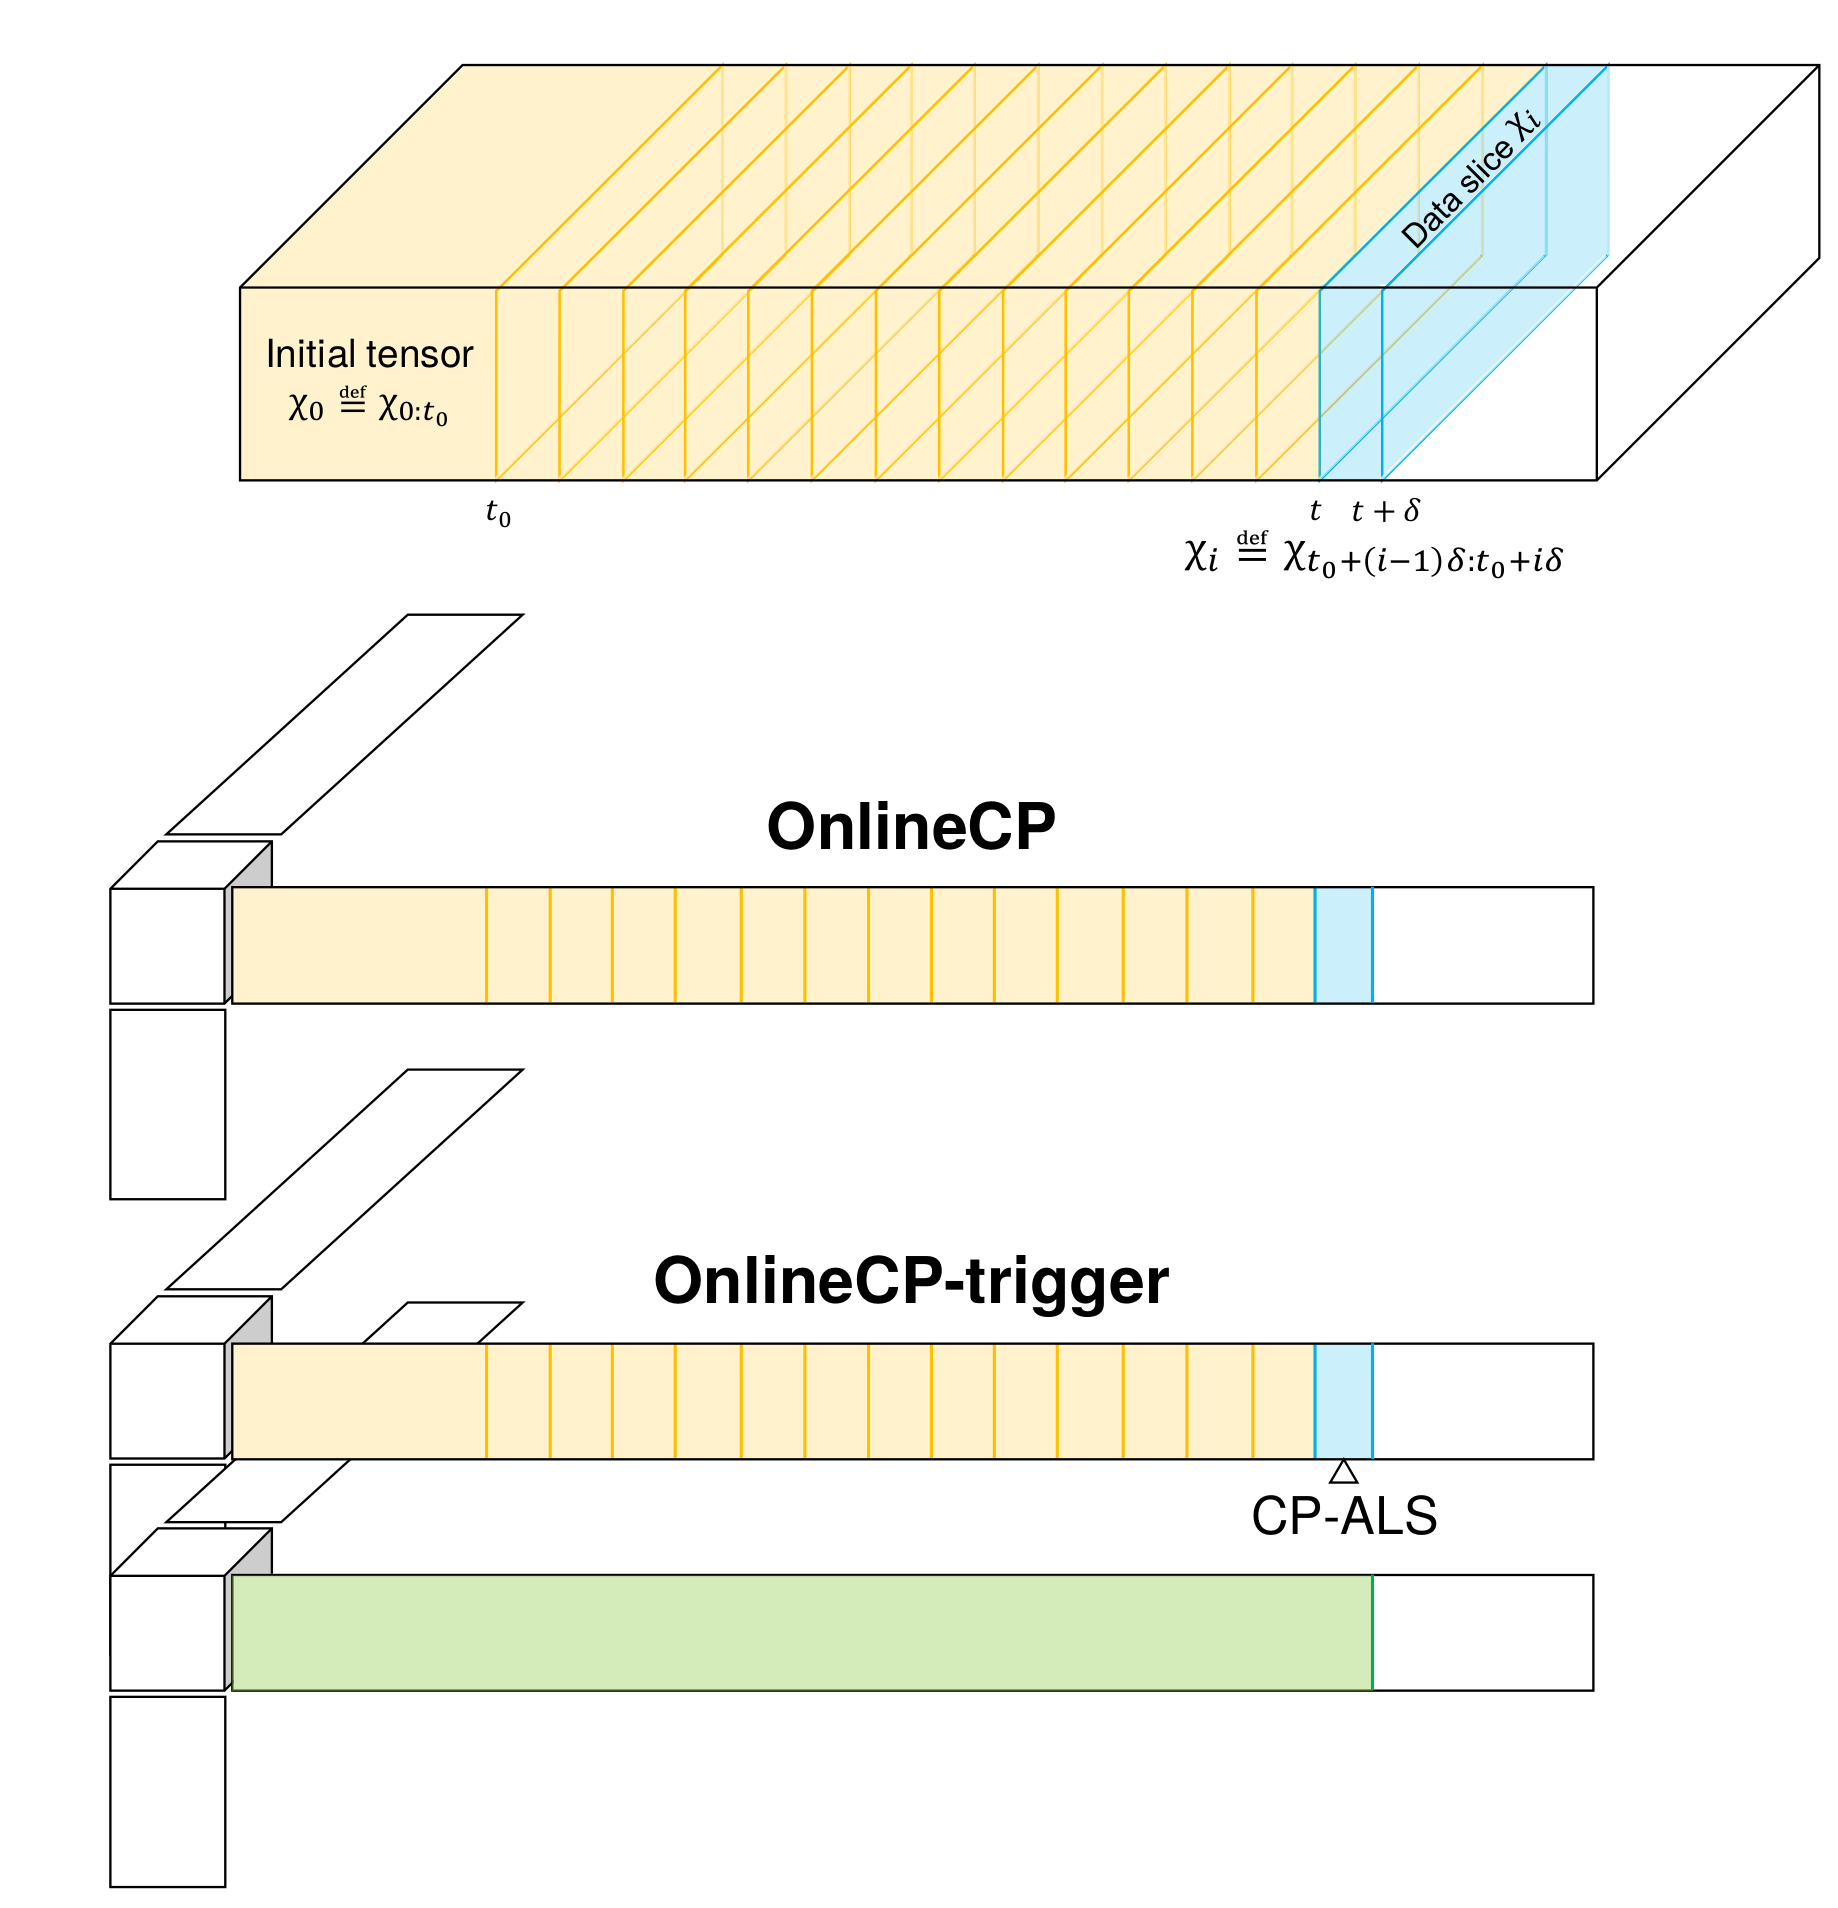
\includegraphics[width=0.85\textwidth]{FIG/OnlineCP-trigger.png}
\end{center}

\newpage
\subsection{\em OnlineCP-split}
\textbf{Split Approach}: trigger function in detection approach tells us sudden change in data. What if the incoming data may have a new theme unseen before? It implies that new decomposition starting point with tensor split is needed. In this approach, we'd like to apply the trigger function for splitting the tensor into serial tensors of different themes. (e.g. $A$, $B$, $C$, $D$)

\begin{center}
	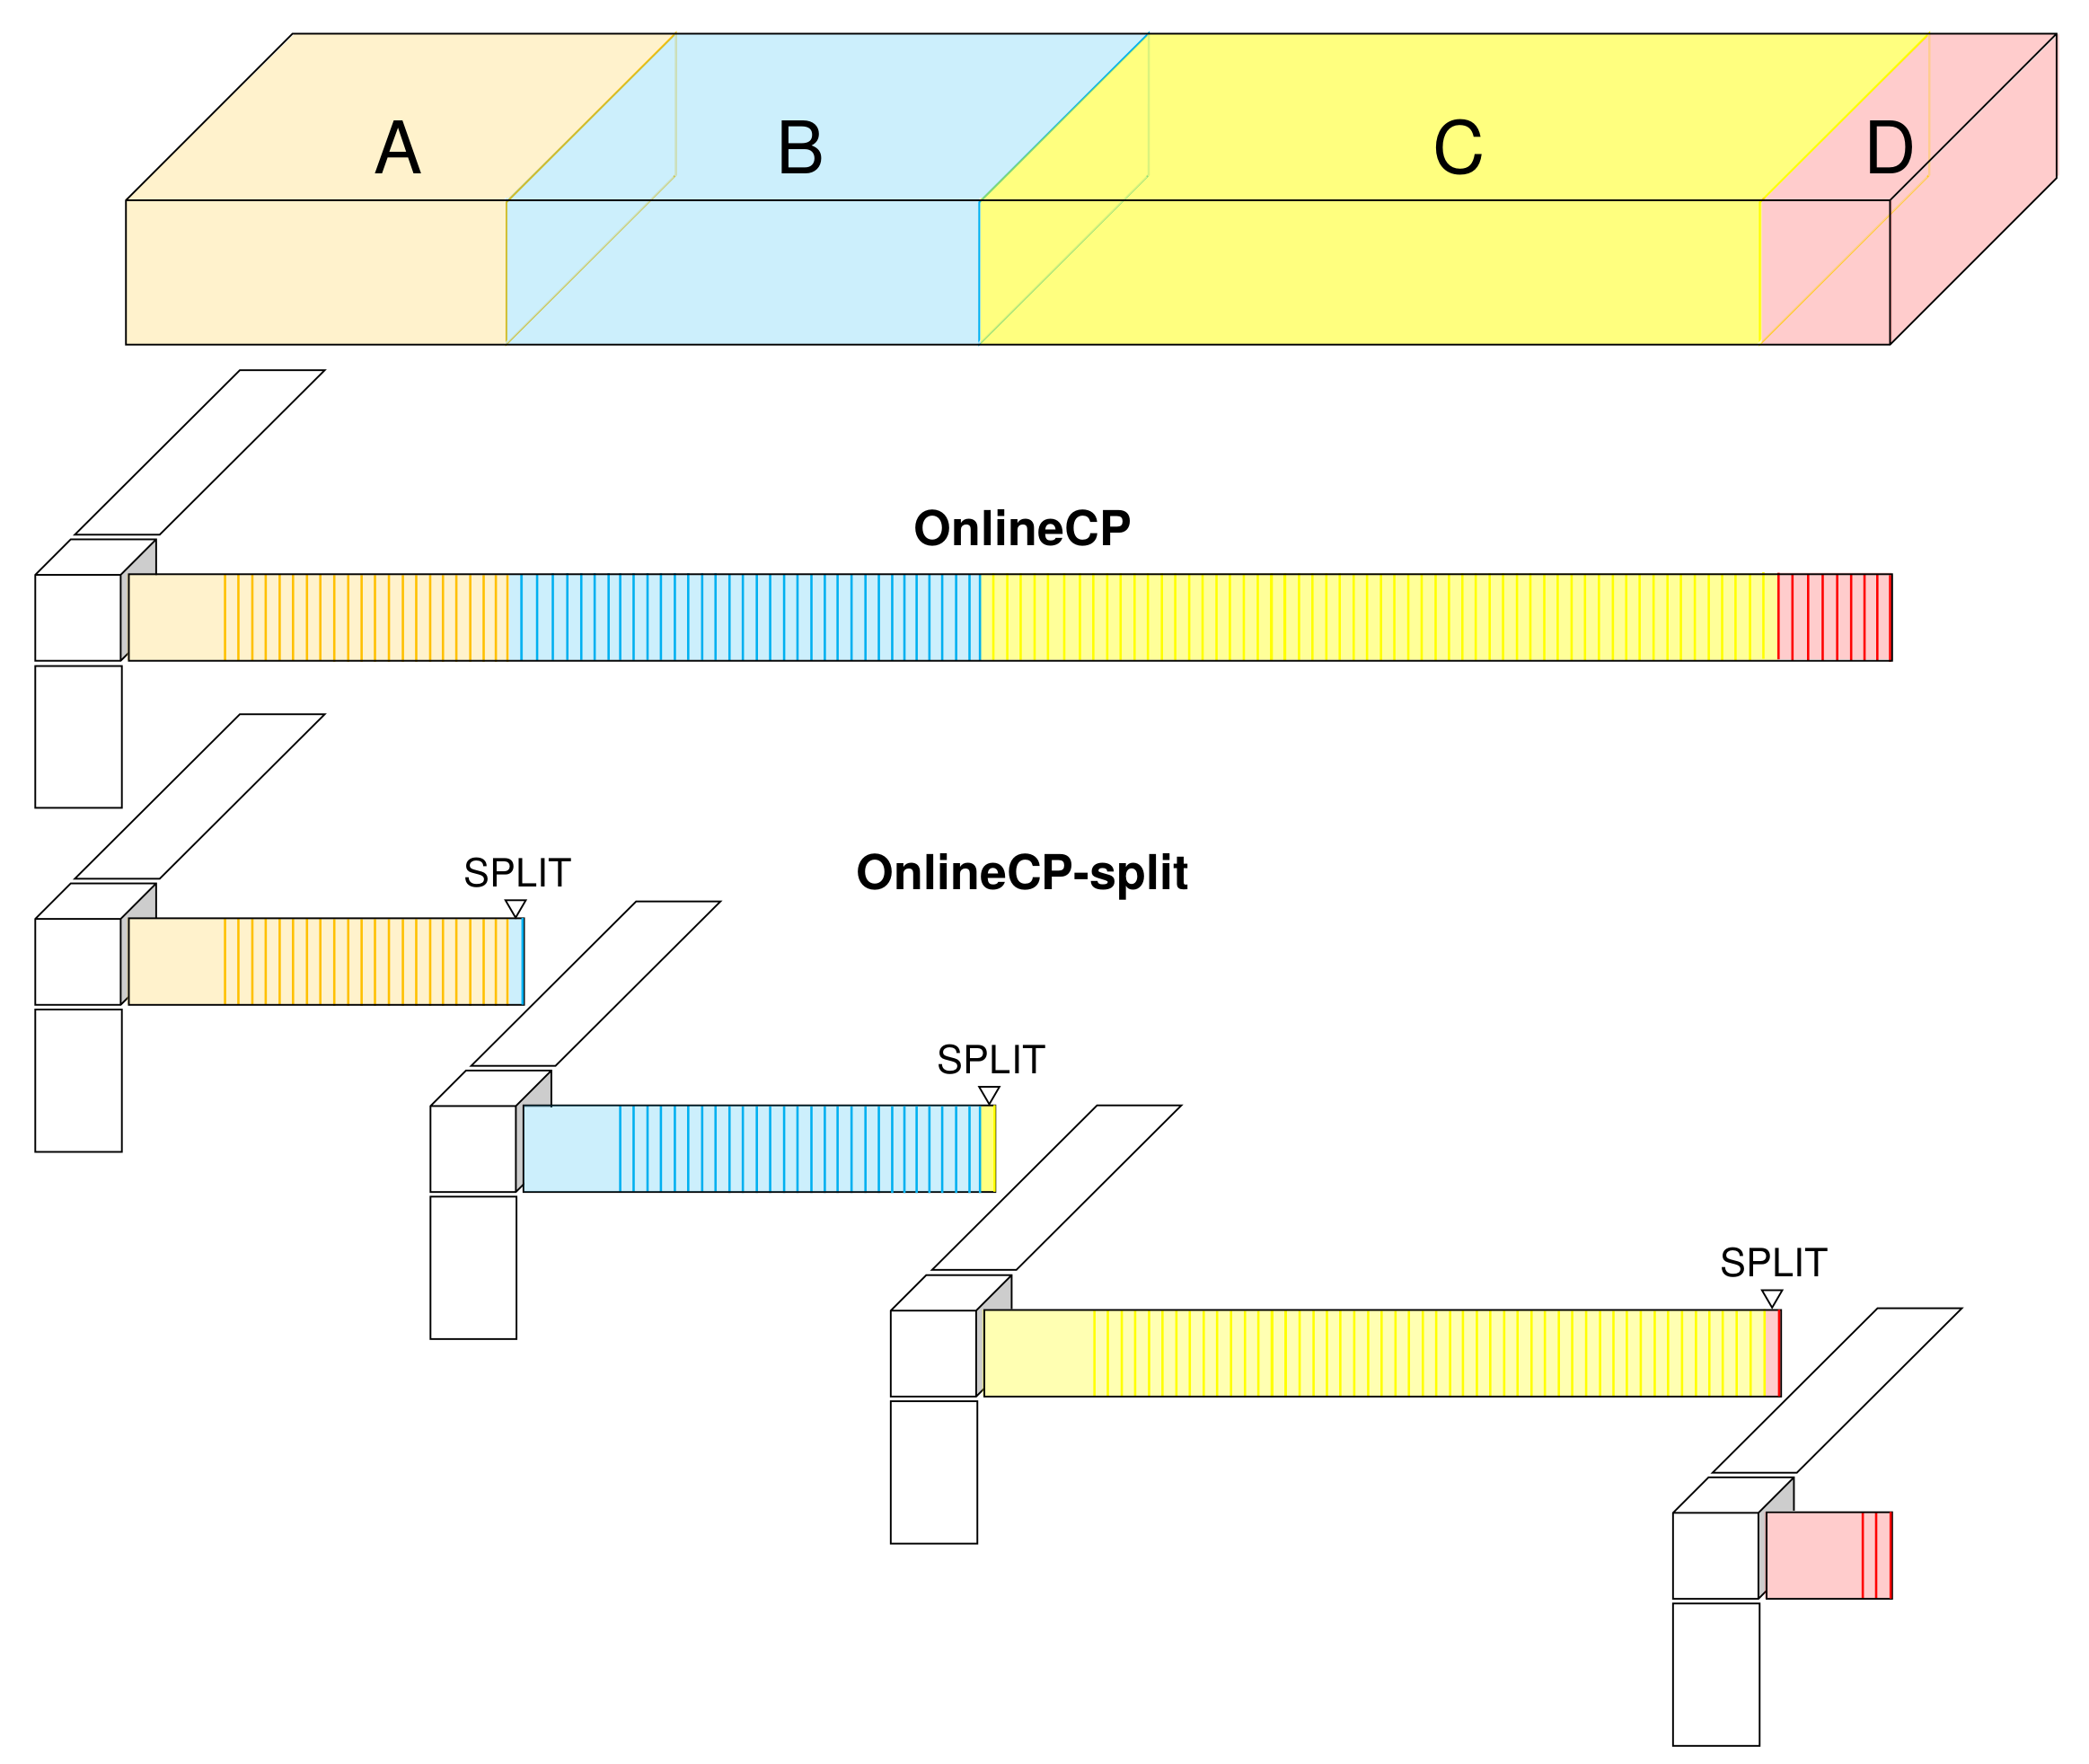
\includegraphics[width=0.9\textwidth]{FIG/OnlineCP-split.png}
\end{center}

\newpage
\subsection{\em OnlineCP-select}
\textbf{Selection Approach}: Similarly to split approach, trigger function now decides whether to split or to concatenate behind after one temporal factor update. It allows to store the tensor efficiently; group tensors with similar themes and split them otherwise. (e.g. $A$, $B$, $B’$, $C$)

\begin{center}
	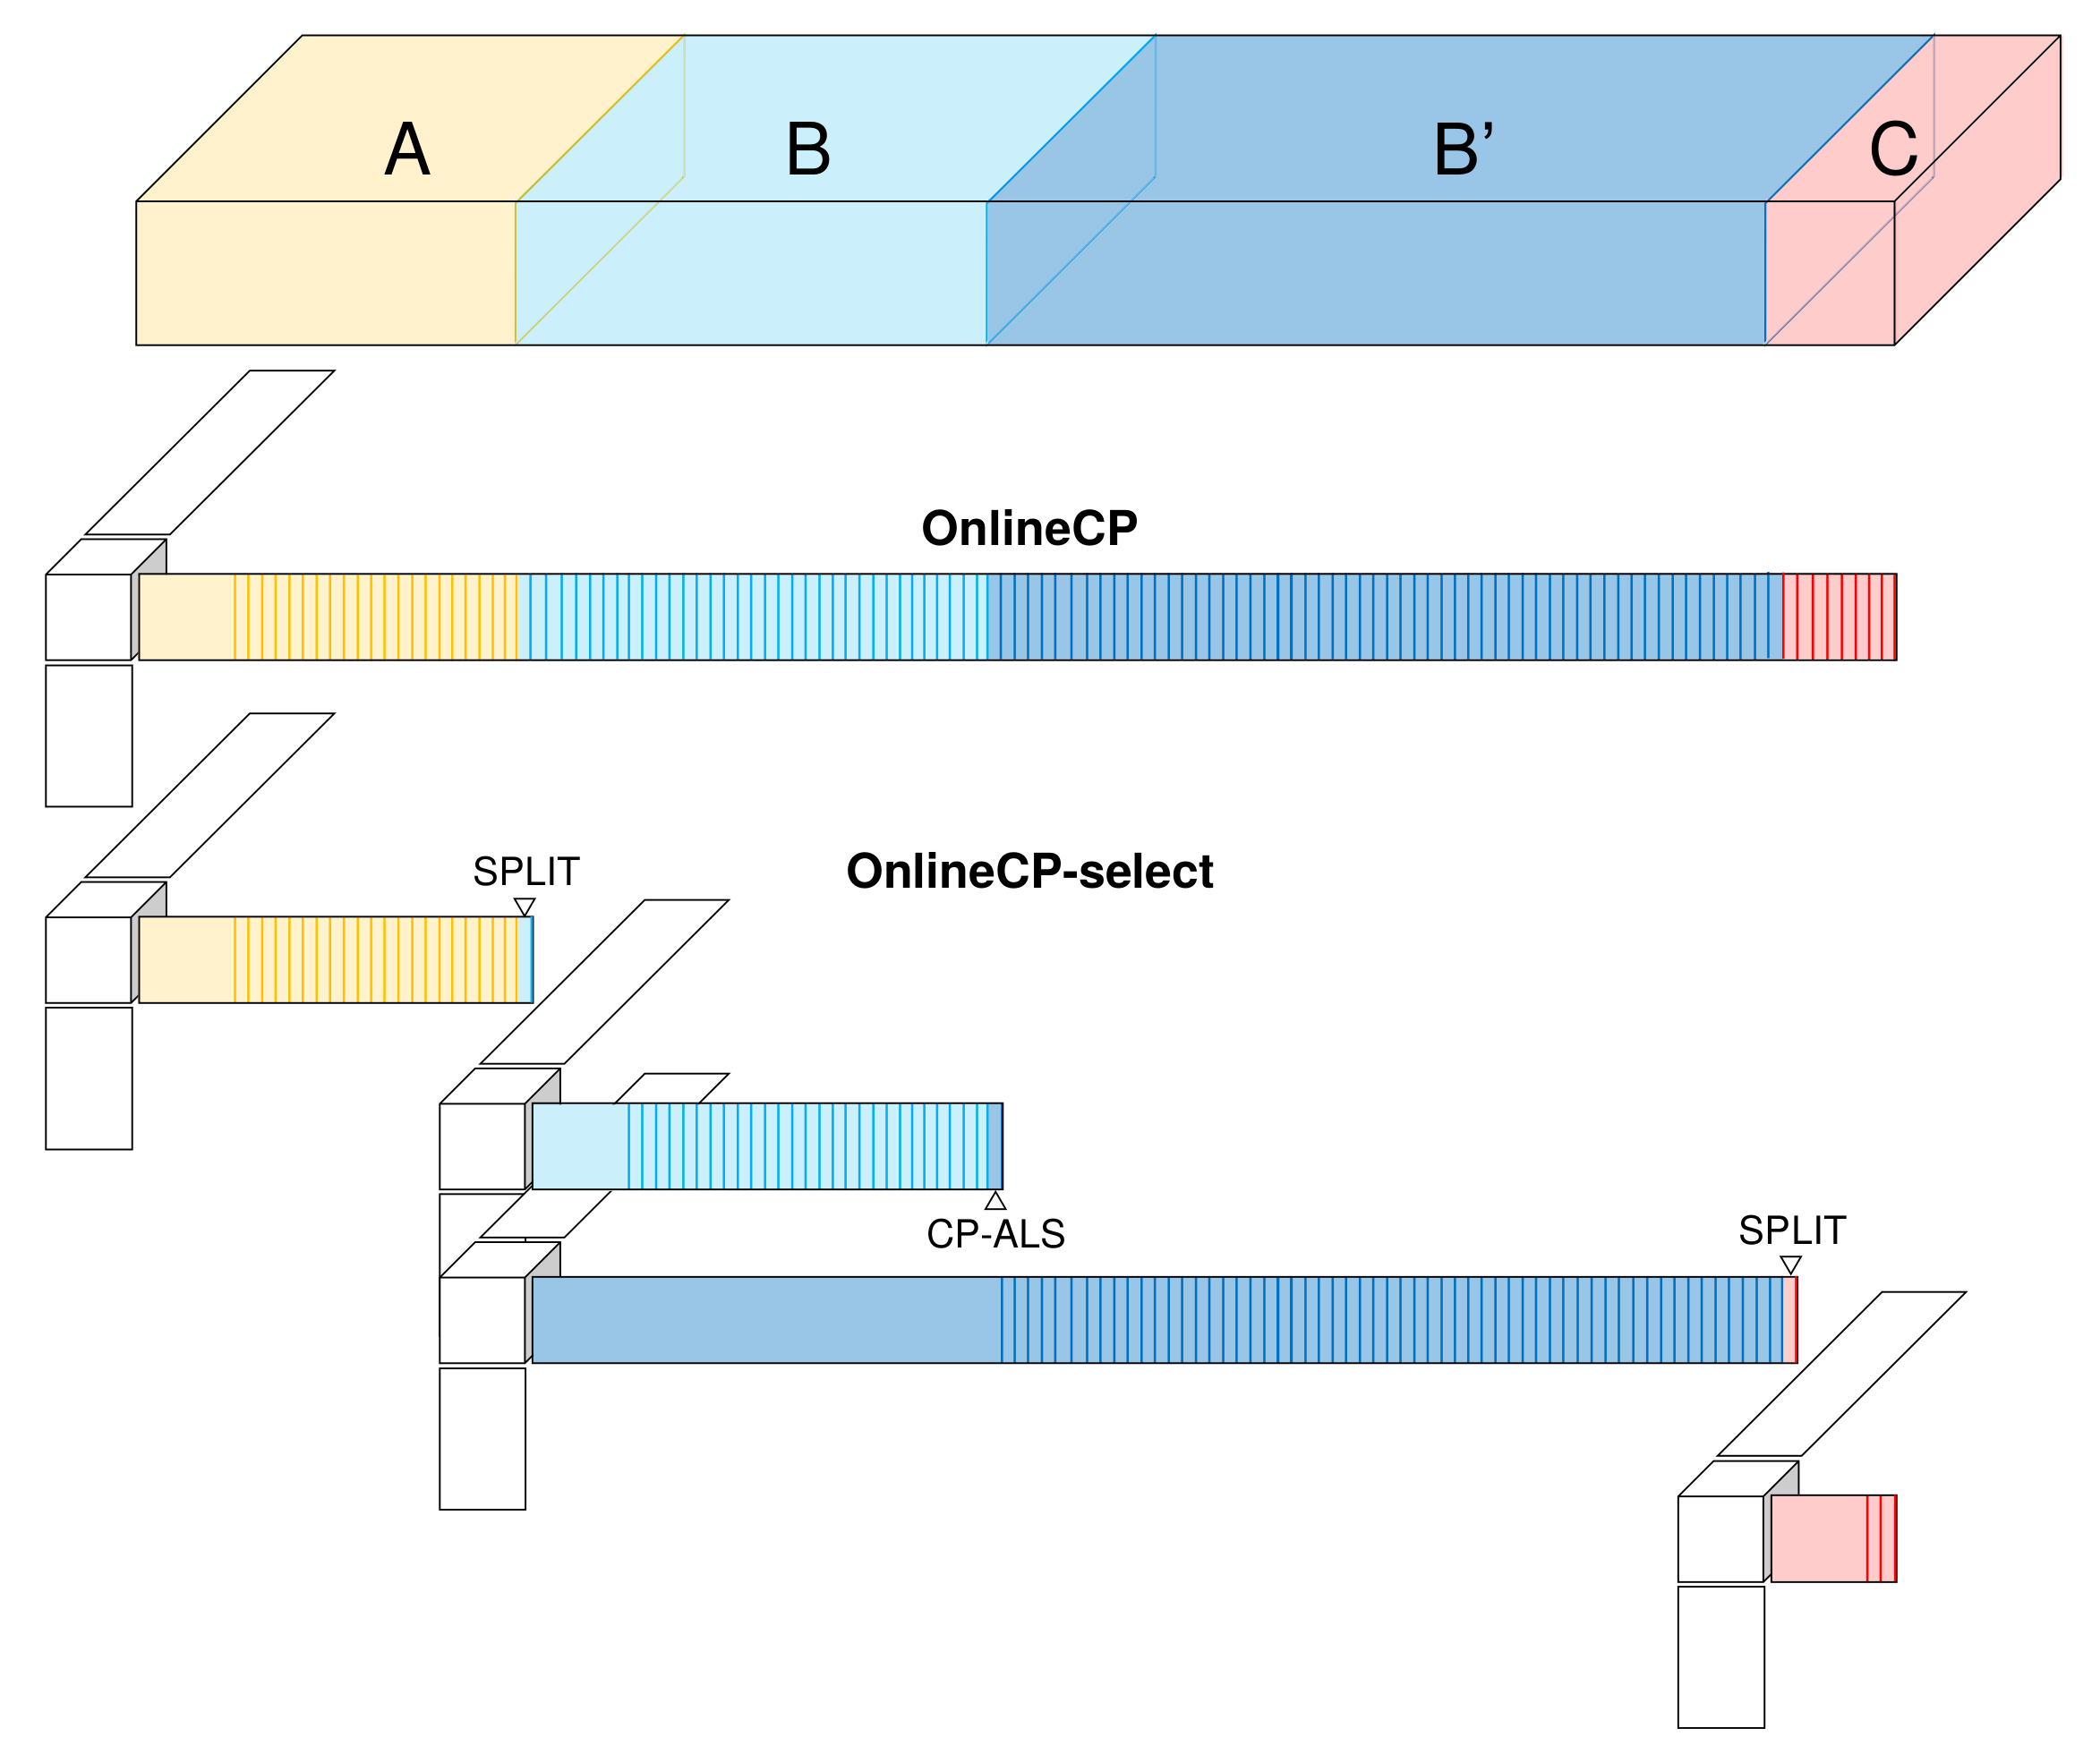
\includegraphics[width=0.9\textwidth]{FIG/OnlineCP-select.png}
\end{center}